\documentclass[]{article}
\usepackage{lmodern}
\usepackage{amssymb,amsmath}
\usepackage{ifxetex,ifluatex}
\usepackage{fixltx2e} % provides \textsubscript
\ifnum 0\ifxetex 1\fi\ifluatex 1\fi=0 % if pdftex
  \usepackage[T1]{fontenc}
  \usepackage[utf8]{inputenc}
\else % if luatex or xelatex
  \ifxetex
    \usepackage{mathspec}
  \else
    \usepackage{fontspec}
  \fi
  \defaultfontfeatures{Ligatures=TeX,Scale=MatchLowercase}
\fi
% use upquote if available, for straight quotes in verbatim environments
\IfFileExists{upquote.sty}{\usepackage{upquote}}{}
% use microtype if available
\IfFileExists{microtype.sty}{%
\usepackage[]{microtype}
\UseMicrotypeSet[protrusion]{basicmath} % disable protrusion for tt fonts
}{}
\PassOptionsToPackage{hyphens}{url} % url is loaded by hyperref
\usepackage[unicode=true]{hyperref}
\hypersetup{
            pdfborder={0 0 0},
            breaklinks=true}
\urlstyle{same}  % don't use monospace font for urls
\usepackage[margin=1in]{geometry}
\usepackage{color}
\usepackage{fancyvrb}
\newcommand{\VerbBar}{|}
\newcommand{\VERB}{\Verb[commandchars=\\\{\}]}
\DefineVerbatimEnvironment{Highlighting}{Verbatim}{commandchars=\\\{\}}
% Add ',fontsize=\small' for more characters per line
\usepackage{framed}
\definecolor{shadecolor}{RGB}{248,248,248}
\newenvironment{Shaded}{\begin{snugshade}}{\end{snugshade}}
\newcommand{\KeywordTok}[1]{\textcolor[rgb]{0.13,0.29,0.53}{\textbf{#1}}}
\newcommand{\DataTypeTok}[1]{\textcolor[rgb]{0.13,0.29,0.53}{#1}}
\newcommand{\DecValTok}[1]{\textcolor[rgb]{0.00,0.00,0.81}{#1}}
\newcommand{\BaseNTok}[1]{\textcolor[rgb]{0.00,0.00,0.81}{#1}}
\newcommand{\FloatTok}[1]{\textcolor[rgb]{0.00,0.00,0.81}{#1}}
\newcommand{\ConstantTok}[1]{\textcolor[rgb]{0.00,0.00,0.00}{#1}}
\newcommand{\CharTok}[1]{\textcolor[rgb]{0.31,0.60,0.02}{#1}}
\newcommand{\SpecialCharTok}[1]{\textcolor[rgb]{0.00,0.00,0.00}{#1}}
\newcommand{\StringTok}[1]{\textcolor[rgb]{0.31,0.60,0.02}{#1}}
\newcommand{\VerbatimStringTok}[1]{\textcolor[rgb]{0.31,0.60,0.02}{#1}}
\newcommand{\SpecialStringTok}[1]{\textcolor[rgb]{0.31,0.60,0.02}{#1}}
\newcommand{\ImportTok}[1]{#1}
\newcommand{\CommentTok}[1]{\textcolor[rgb]{0.56,0.35,0.01}{\textit{#1}}}
\newcommand{\DocumentationTok}[1]{\textcolor[rgb]{0.56,0.35,0.01}{\textbf{\textit{#1}}}}
\newcommand{\AnnotationTok}[1]{\textcolor[rgb]{0.56,0.35,0.01}{\textbf{\textit{#1}}}}
\newcommand{\CommentVarTok}[1]{\textcolor[rgb]{0.56,0.35,0.01}{\textbf{\textit{#1}}}}
\newcommand{\OtherTok}[1]{\textcolor[rgb]{0.56,0.35,0.01}{#1}}
\newcommand{\FunctionTok}[1]{\textcolor[rgb]{0.00,0.00,0.00}{#1}}
\newcommand{\VariableTok}[1]{\textcolor[rgb]{0.00,0.00,0.00}{#1}}
\newcommand{\ControlFlowTok}[1]{\textcolor[rgb]{0.13,0.29,0.53}{\textbf{#1}}}
\newcommand{\OperatorTok}[1]{\textcolor[rgb]{0.81,0.36,0.00}{\textbf{#1}}}
\newcommand{\BuiltInTok}[1]{#1}
\newcommand{\ExtensionTok}[1]{#1}
\newcommand{\PreprocessorTok}[1]{\textcolor[rgb]{0.56,0.35,0.01}{\textit{#1}}}
\newcommand{\AttributeTok}[1]{\textcolor[rgb]{0.77,0.63,0.00}{#1}}
\newcommand{\RegionMarkerTok}[1]{#1}
\newcommand{\InformationTok}[1]{\textcolor[rgb]{0.56,0.35,0.01}{\textbf{\textit{#1}}}}
\newcommand{\WarningTok}[1]{\textcolor[rgb]{0.56,0.35,0.01}{\textbf{\textit{#1}}}}
\newcommand{\AlertTok}[1]{\textcolor[rgb]{0.94,0.16,0.16}{#1}}
\newcommand{\ErrorTok}[1]{\textcolor[rgb]{0.64,0.00,0.00}{\textbf{#1}}}
\newcommand{\NormalTok}[1]{#1}
\usepackage{graphicx,grffile}
\makeatletter
\def\maxwidth{\ifdim\Gin@nat@width>\linewidth\linewidth\else\Gin@nat@width\fi}
\def\maxheight{\ifdim\Gin@nat@height>\textheight\textheight\else\Gin@nat@height\fi}
\makeatother
% Scale images if necessary, so that they will not overflow the page
% margins by default, and it is still possible to overwrite the defaults
% using explicit options in \includegraphics[width, height, ...]{}
\setkeys{Gin}{width=\maxwidth,height=\maxheight,keepaspectratio}
\IfFileExists{parskip.sty}{%
\usepackage{parskip}
}{% else
\setlength{\parindent}{0pt}
\setlength{\parskip}{6pt plus 2pt minus 1pt}
}
\setlength{\emergencystretch}{3em}  % prevent overfull lines
\providecommand{\tightlist}{%
  \setlength{\itemsep}{0pt}\setlength{\parskip}{0pt}}
\setcounter{secnumdepth}{0}
% Redefines (sub)paragraphs to behave more like sections
\ifx\paragraph\undefined\else
\let\oldparagraph\paragraph
\renewcommand{\paragraph}[1]{\oldparagraph{#1}\mbox{}}
\fi
\ifx\subparagraph\undefined\else
\let\oldsubparagraph\subparagraph
\renewcommand{\subparagraph}[1]{\oldsubparagraph{#1}\mbox{}}
\fi

% set default figure placement to htbp
\makeatletter
\def\fps@figure{htbp}
\makeatother


\author{}
\date{\vspace{-2.5em}}

\begin{document}

\section{Assignment 1 - Reprodusible
Research}\label{assignment-1---reprodusible-research}

\begin{enumerate}
\def\labelenumi{\arabic{enumi})}
\tightlist
\item
  Loading and preprocessing the data
\end{enumerate}

The data is downloaded from the website and is located on the
corresponding folder. Afterwards, it's unzipped and the missing values
are ommited.

\begin{Shaded}
\begin{Highlighting}[]
\NormalTok{file <-}\StringTok{ "repdata_data_activity.zip"}
\ControlFlowTok{if}\NormalTok{ (}\OperatorTok{!}\KeywordTok{file.exists}\NormalTok{(file)) \{}
\NormalTok{  download <-}\StringTok{ "https://d396qusza40orc.cloudfront.net/repdata%2Fdata%2Factivity.zip"}
 \KeywordTok{download.file}\NormalTok{(download, }\DataTypeTok{destfile =}\NormalTok{ file)}
 \KeywordTok{unzip}\NormalTok{ (}\DataTypeTok{zipfile =}\NormalTok{ file)}
\NormalTok{\}}
\NormalTok{data_original_form <-}\StringTok{ }\KeywordTok{read.csv}\NormalTok{(}\StringTok{"activity.csv"}\NormalTok{, }\DataTypeTok{header =} \OtherTok{TRUE}\NormalTok{)}
\NormalTok{working_data <-}\StringTok{ }\KeywordTok{na.omit}\NormalTok{(data_original_form)}
\KeywordTok{head}\NormalTok{(working_data)}
\end{Highlighting}
\end{Shaded}

\begin{verbatim}
##     steps       date interval
## 289     0 2012-10-02        0
## 290     0 2012-10-02        5
## 291     0 2012-10-02       10
## 292     0 2012-10-02       15
## 293     0 2012-10-02       20
## 294     0 2012-10-02       25
\end{verbatim}

\begin{enumerate}
\def\labelenumi{\arabic{enumi})}
\setcounter{enumi}{1}
\tightlist
\item
  What is mean total number of steps taken per day?
\end{enumerate}

First, the total number of daily steps is calculated by aggregating the
steps for each day

\begin{Shaded}
\begin{Highlighting}[]
\NormalTok{steps_day <-}\StringTok{ }\KeywordTok{aggregate}\NormalTok{(working_data}\OperatorTok{$}\NormalTok{steps, }\DataTypeTok{by =} \KeywordTok{list}\NormalTok{(}\DataTypeTok{Steps.Date =}\NormalTok{ working_data}\OperatorTok{$}\NormalTok{date), }\DataTypeTok{FUN =} \StringTok{"sum"}\NormalTok{)}
\end{Highlighting}
\end{Shaded}

Second, a histogram is constructed, which shows the frequency of the
different number of steps per day

\begin{Shaded}
\begin{Highlighting}[]
\KeywordTok{hist}\NormalTok{(steps_day}\OperatorTok{$}\NormalTok{x, }\DataTypeTok{col =} \StringTok{"blue"}\NormalTok{, }
     \DataTypeTok{breaks =} \DecValTok{30}\NormalTok{,}
     \DataTypeTok{main =} \StringTok{"Steps taken in each day"}\NormalTok{,}
     \DataTypeTok{xlab =} \StringTok{"Steps per day"}\NormalTok{)}
\end{Highlighting}
\end{Shaded}

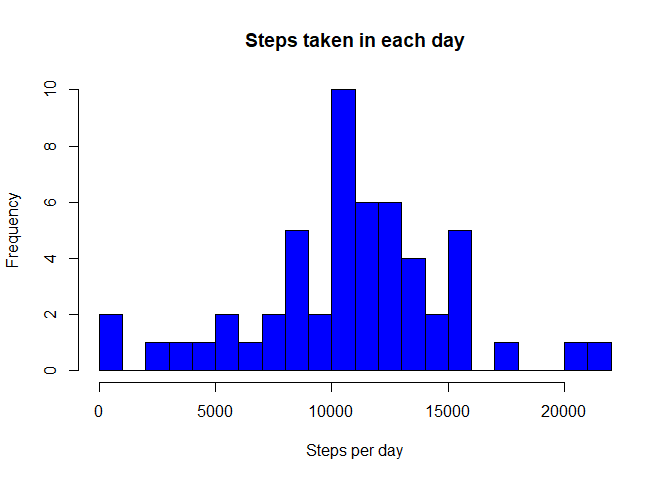
\includegraphics{Markdown_demo_files/figure-latex/unnamed-chunk-3-1.pdf}

The mean and median number of steps are calculated. Here we observe that
they are slightly different.

\begin{Shaded}
\begin{Highlighting}[]
\KeywordTok{mean}\NormalTok{(steps_day[,}\DecValTok{2}\NormalTok{], }\DataTypeTok{na.rm =} \OtherTok{TRUE}\NormalTok{)}
\end{Highlighting}
\end{Shaded}

\begin{verbatim}
## [1] 10766.19
\end{verbatim}

\begin{Shaded}
\begin{Highlighting}[]
\KeywordTok{median}\NormalTok{(steps_day[,}\DecValTok{2}\NormalTok{], }\DataTypeTok{na.rm =} \OtherTok{TRUE}\NormalTok{)}
\end{Highlighting}
\end{Shaded}

\begin{verbatim}
## [1] 10765
\end{verbatim}

\begin{enumerate}
\def\labelenumi{\arabic{enumi})}
\setcounter{enumi}{2}
\tightlist
\item
  What is the average daily activity pattern?
\end{enumerate}

The average daily activity pattern is obtained by calculating the mean
of the steps for each 5-minute interval.

\begin{Shaded}
\begin{Highlighting}[]
\NormalTok{average_activity <-}\StringTok{ }\KeywordTok{aggregate}\NormalTok{(working_data}\OperatorTok{$}\NormalTok{steps, }
                          \DataTypeTok{by =} \KeywordTok{list}\NormalTok{(}\DataTypeTok{Interval =}\NormalTok{ working_data}\OperatorTok{$}\NormalTok{interval), }
                          \DataTypeTok{FUN =} \StringTok{"mean"}\NormalTok{)}
\KeywordTok{plot}\NormalTok{(average_activity}\OperatorTok{$}\NormalTok{Interval, average_activity}\OperatorTok{$}\NormalTok{x, }\DataTypeTok{type =} \StringTok{"l"}\NormalTok{, }
     \DataTypeTok{main =} \StringTok{"Average daily activity"}\NormalTok{, }
     \DataTypeTok{ylab =} \StringTok{"Avarage steps"}\NormalTok{, }
     \DataTypeTok{xlab =} \StringTok{"5 minutes intervals"}\NormalTok{)}
\end{Highlighting}
\end{Shaded}

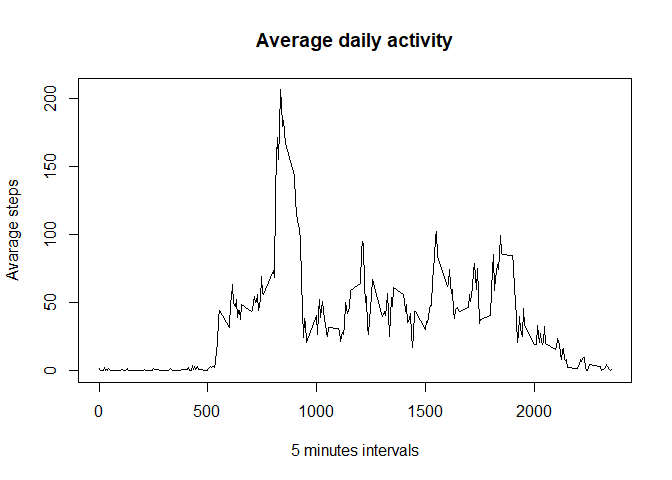
\includegraphics{Markdown_demo_files/figure-latex/unnamed-chunk-5-1.pdf}

Which 5-minute interval, on average across all the days in the dataset,
contains the maximum number of steps?

Afterwards, we identify the 5-minute interval which is associated with
the maximum number of average steps.

\begin{Shaded}
\begin{Highlighting}[]
\NormalTok{interval_max <-}\StringTok{ }\KeywordTok{which.max}\NormalTok{(average_activity}\OperatorTok{$}\NormalTok{x)}
\NormalTok{max_interval <-}\StringTok{ }\NormalTok{average_activity[interval_max,}\DecValTok{1}\NormalTok{]}
\KeywordTok{print}\NormalTok{ (max_interval)}
\end{Highlighting}
\end{Shaded}

\begin{verbatim}
## [1] 835
\end{verbatim}

\begin{enumerate}
\def\labelenumi{\arabic{enumi})}
\setcounter{enumi}{3}
\tightlist
\item
  Imputing missing values
\end{enumerate}

The number of missing values is identified and tabulated.

\begin{Shaded}
\begin{Highlighting}[]
\NormalTok{missing_values <-}\StringTok{ }\KeywordTok{is.na}\NormalTok{(data_original_form}\OperatorTok{$}\NormalTok{steps)}
\KeywordTok{table}\NormalTok{(missing_values)}
\end{Highlighting}
\end{Shaded}

\begin{verbatim}
## missing_values
## FALSE  TRUE 
## 15264  2304
\end{verbatim}

The missing values are imputed with the mean for the 5-min interval
using the HMISC package.

\begin{Shaded}
\begin{Highlighting}[]
\KeywordTok{library}\NormalTok{(Hmisc)}
\end{Highlighting}
\end{Shaded}

\begin{verbatim}
## Warning: package 'Hmisc' was built under R version 4.0.5
\end{verbatim}

\begin{verbatim}
## Loading required package: lattice
\end{verbatim}

\begin{verbatim}
## Loading required package: survival
\end{verbatim}

\begin{verbatim}
## Loading required package: Formula
\end{verbatim}

\begin{verbatim}
## Loading required package: ggplot2
\end{verbatim}

\begin{verbatim}
## Warning: package 'ggplot2' was built under R version 4.0.5
\end{verbatim}

\begin{verbatim}
## 
## Attaching package: 'Hmisc'
\end{verbatim}

\begin{verbatim}
## The following objects are masked from 'package:base':
## 
##     format.pval, units
\end{verbatim}

\begin{Shaded}
\begin{Highlighting}[]
\NormalTok{original_data_filled <-}\StringTok{ }\NormalTok{data_original_form}
\NormalTok{original_data_filled}\OperatorTok{$}\NormalTok{steps <-}\StringTok{ }\KeywordTok{impute}\NormalTok{(data_original_form}\OperatorTok{$}\NormalTok{steps, }\DataTypeTok{fun=}\NormalTok{mean)}
\KeywordTok{head}\NormalTok{(original_data_filled)}
\end{Highlighting}
\end{Shaded}

\begin{verbatim}
##     steps       date interval
## 1 37.3826 2012-10-01        0
## 2 37.3826 2012-10-01        5
## 3 37.3826 2012-10-01       10
## 4 37.3826 2012-10-01       15
## 5 37.3826 2012-10-01       20
## 6 37.3826 2012-10-01       25
\end{verbatim}

The histogram of the total number of steps generated with the new
imputed database is calculated.

\begin{Shaded}
\begin{Highlighting}[]
\NormalTok{steps_day_imputed <-}\StringTok{ }\KeywordTok{aggregate}\NormalTok{(original_data_filled}\OperatorTok{$}\NormalTok{steps, }\DataTypeTok{by =} \KeywordTok{list}\NormalTok{(}\DataTypeTok{Steps.Date =}\NormalTok{ original_data_filled}\OperatorTok{$}\NormalTok{date), }\DataTypeTok{FUN =} \StringTok{"sum"}\NormalTok{)}
\KeywordTok{hist}\NormalTok{(steps_day_imputed}\OperatorTok{$}\NormalTok{x, }\DataTypeTok{col =} \StringTok{"blue"}\NormalTok{, }
     \DataTypeTok{breaks =} \DecValTok{30}\NormalTok{,}
     \DataTypeTok{main =} \StringTok{"Steps taken in each day"}\NormalTok{,}
     \DataTypeTok{xlab =} \StringTok{"Steps per day"}\NormalTok{)}
\end{Highlighting}
\end{Shaded}

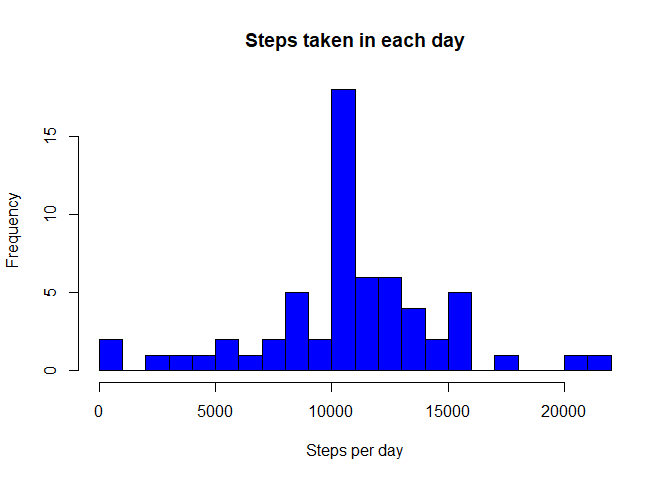
\includegraphics{Markdown_demo_files/figure-latex/unnamed-chunk-9-1.pdf}

The mean and the median are reported, which right now are equal.

\begin{Shaded}
\begin{Highlighting}[]
\KeywordTok{mean}\NormalTok{(steps_day_imputed[,}\DecValTok{2}\NormalTok{], }\DataTypeTok{na.rm =} \OtherTok{TRUE}\NormalTok{)}
\end{Highlighting}
\end{Shaded}

\begin{verbatim}
## [1] 10766.19
\end{verbatim}

\begin{Shaded}
\begin{Highlighting}[]
\KeywordTok{median}\NormalTok{(steps_day_imputed[,}\DecValTok{2}\NormalTok{], }\DataTypeTok{na.rm =} \OtherTok{TRUE}\NormalTok{)}
\end{Highlighting}
\end{Shaded}

\begin{verbatim}
## [1] 10766.19
\end{verbatim}

\begin{enumerate}
\def\labelenumi{\arabic{enumi})}
\setcounter{enumi}{4}
\tightlist
\item
  Are there differences in activity patterns between weekdays and
  weekends?
\end{enumerate}

A new factor variable is created. This variable indicates if the
specific date belongs to a weekday or a weekend.

\begin{Shaded}
\begin{Highlighting}[]
\NormalTok{original_data_filled}\OperatorTok{$}\NormalTok{date <-}\StringTok{ }\KeywordTok{as.Date}\NormalTok{(}\KeywordTok{strptime}\NormalTok{(original_data_filled}\OperatorTok{$}\NormalTok{date, }\DataTypeTok{format=}\StringTok{"%Y-%m-%d"}\NormalTok{))}
\NormalTok{original_data_filled}\OperatorTok{$}\NormalTok{datetype <-}\StringTok{ }\KeywordTok{sapply}\NormalTok{(original_data_filled}\OperatorTok{$}\NormalTok{date, }\ControlFlowTok{function}\NormalTok{(x) \{}
  \ControlFlowTok{if}\NormalTok{ (}\KeywordTok{weekdays}\NormalTok{(x) }\OperatorTok{==}\StringTok{ "Saturday"} \OperatorTok{|}\StringTok{ }\KeywordTok{weekdays}\NormalTok{(x) }\OperatorTok{==}\StringTok{"Sunday"}\NormalTok{) }
\NormalTok{  \{y <-}\StringTok{ "Weekend"}\NormalTok{\} }\ControlFlowTok{else} 
\NormalTok{  \{y <-}\StringTok{ "Weekday"}\NormalTok{\}}
\NormalTok{  y}
\NormalTok{\})}
\KeywordTok{head}\NormalTok{(original_data_filled)}
\end{Highlighting}
\end{Shaded}

\begin{verbatim}
##     steps       date interval datetype
## 1 37.3826 2012-10-01        0  Weekday
## 2 37.3826 2012-10-01        5  Weekday
## 3 37.3826 2012-10-01       10  Weekday
## 4 37.3826 2012-10-01       15  Weekday
## 5 37.3826 2012-10-01       20  Weekday
## 6 37.3826 2012-10-01       25  Weekday
\end{verbatim}

Finally, time series plot showing the average number of steps (y axis)
by interval (x axis) for weekdays and weekends are generated

\begin{Shaded}
\begin{Highlighting}[]
\NormalTok{activity_date <-}\StringTok{ }\KeywordTok{aggregate}\NormalTok{(steps}\OperatorTok{~}\NormalTok{interval }\OperatorTok{+}\StringTok{ }\NormalTok{datetype, original_data_filled, mean, }\DataTypeTok{na.rm =} \OtherTok{TRUE}\NormalTok{)}
\NormalTok{plot<-}\StringTok{ }\KeywordTok{ggplot}\NormalTok{(activity_date, }\KeywordTok{aes}\NormalTok{(}\DataTypeTok{x =}\NormalTok{ interval , }\DataTypeTok{y =}\NormalTok{ steps, }\DataTypeTok{color =}\NormalTok{ datetype)) }\OperatorTok{+}
\StringTok{  }\KeywordTok{geom_line}\NormalTok{() }\OperatorTok{+}
\StringTok{  }\KeywordTok{labs}\NormalTok{(}\DataTypeTok{title =} \StringTok{"Average daily steps by weekday or weekend"}\NormalTok{, }\DataTypeTok{x =} \StringTok{"Interval"}\NormalTok{, }\DataTypeTok{y =} \StringTok{"Average n. of steps"}\NormalTok{) }\OperatorTok{+}
\StringTok{  }\KeywordTok{facet_wrap}\NormalTok{(}\OperatorTok{~}\NormalTok{datetype, }\DataTypeTok{ncol =} \DecValTok{1}\NormalTok{, }\DataTypeTok{nrow=}\DecValTok{2}\NormalTok{)}
\KeywordTok{print}\NormalTok{(plot)}
\end{Highlighting}
\end{Shaded}

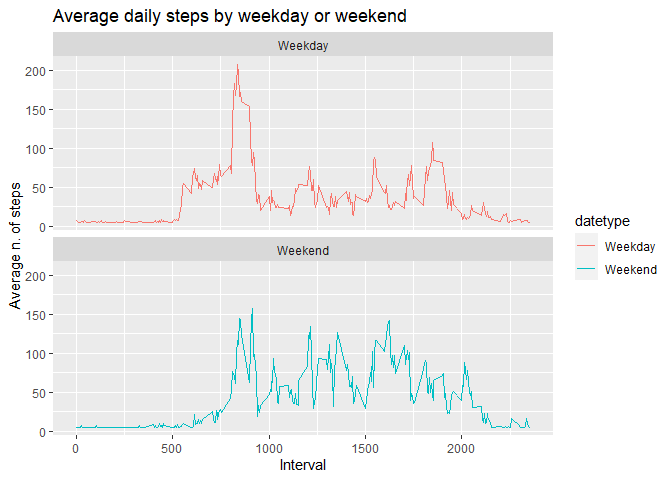
\includegraphics{Markdown_demo_files/figure-latex/unnamed-chunk-12-1.pdf}

\end{document}
